\chapter{System Overview}
\pagenumbering{arabic}


\section{What is \GrG?}

\GrG\ (\textsc{G}raph \textsc{R}ewrite \textsc{Gen}arator) is a generative programming system for graph rewriting, which applies heuristic optimizations to the matching problem.
According to Varr\'o's benchmark it is at least one order of magnitude faster than any other tool known to us.

For the rewriting step, our tool implements the well-founded single-pushout approach (SPO, for explanation see \cite{spo}).
In order to accelerating the matching step, we define the notion of search plans to represent different matching strategies and equip these search plans with a cost model, taking the present host graph into account.
The task of selecting a good search plan is then viewed as an optimization problem.

For the ease of use, \GrG\ features an expressive specification language and generates program code with a convenient interface.
In contrast to systems like Fujaba our pattern matching algorithm is fully automatic and does not need be tuned or partly be implemented by hand.


\section{Features of \GrG}

The process of graph rewriting can be divied into four step: 
Representing a graph according to a model, searching a pattern aka.\ finding a match, performing changes to the found match and, finally, selecting the next rule(s) for application.
We have organiced the features of \GrG\ accoriding to this breakdown of graph rewriting.

\begin{itemize}
  \item Graph model (Meta-Model) supports:
  \begin{itemize}
    \item Directed graphs
    \item Typed nodes and edges, with multiple inheritance on types (see ).
    \item Typed attributes can be assigned to node and edge types (see ).
    \item Multigraphs including multiple edges of the same type
    \item Connection assertions to restrict the "shape" of graphs (see ).
  \end{itemize}
  
  \item Patten language supports:
  \begin{itemize}
    \item Plain isomorphic subgraph matching (injective mapping)
    \item Homomorphic matching for a declarable set of nodes/edges, so that the matching is not injective
    \item Attribute conditions (including arithmetic operations on the attributes)
    \item Type conditions (including powerful instanceof-like type expressions)
    \item Parameter passing to rules
    \item Dynamic patterns with iterative or recursive paths and graphs (yet to be implemented)
  \end{itemize}
  
  \item Rewrites language supports:
  \begin{itemize}
    \item Attribute re-calculation (using arithmetic operations on the attributes)
    \item Retyping of nodes/edges (some kind of casting)
    \item Creation of new nodes/edges with dynamically computed types (some kind of generic templates)
    \item The specification can alternatively express changes to be made to the match or replace the whole match (the semantics is always mapped to SPO)
    \item Returning certain edges/nodes for further computations
  \end{itemize}
  
  \item Rule applications language (\GrShell) supports:
  \begin{itemize}
    \item Composing several rules together with logical and iterative sequence control (called regular graph rewrite sequences, RGS)
    \item Various support for graph/node/edge creation/deletion/input/output
    \item Stepwise and graphic debugging of rule application
    \item Regular graph rewrite sequences can optionally contain nested transactions (yet to be implemented)
  \end{itemize}
  
  \item Alternatively, you can access the matching and rewrite facility through libGr, so you can build your own algorithmic rule applications in a .NET language of your choice. 
\end{itemize}


\section{System Overview}

Figure \ref{figsys} gives an overview of the \GrG\ system components, whereas table \ref{dirstruc} shows the \GrG\ directory structure.
\begin{figure}[htbp]
  \centering
	\scalebox{0.8}{
  \begin{tikzpicture}
      \begin{scope}[shape=rectangle,minimum size=0.75cm,text width=3cm,text centered]
          \tikzstyle{every node}=[draw]
          \node (spec1)    at (0   ,0)    {Rewrite Rules (*.grg)};
          \node (spec2)    at (0   ,2)    {Graph Model (*.gm)};
          \node (grgen)    at (4   ,1)    {\GrG\ Generator (Java, C\#)};
          \node (rewriter) at (10  ,0)    {Rewrite Rules (C\#)};
          \node (types)    at (10  ,2)    {Graph Model (C\#)};
          \node (data)     at (14  ,1)    {Graph Management (C\#)};
          \node (libgr)    at (12  ,4)    {\LibGr (C\#)};
          \node[fill,color=gray] (app)      at (14.1  ,5.6)  {};
          \node[fill=white] (app)      at (14  ,5.5)  {Applications};
          \node (grsh)     at (10  ,5.5)  {\GrShell (C\#)};
          \node (grs)      at (6   ,5.5)  {Graph Rrewrite Script (*.grs)};
      \end{scope}

      \node[draw, minimum width=9cm,minimum height=4cm] (engine) at (12,1) {};
      \node[draw, minimum width=9cm,minimum height=4cm,style=dotted] (ct) at (2,1) {};
      \node[anchor=north east] (engine_lab) at (engine.north east) {Backend (Run Time)};
      \node[anchor=north east] (ct_lab) at (ct.north east) {Frontend (Compile Time)};

      \draw[->,dashed,red,>=triangle 45]     (spec1)   -> (grgen);
      \draw[->,dashed,red,>=triangle 45]     (spec2)   -> (grgen);
      \draw[->,dashed,red,>=triangle 45]     (grgen)   -> (types);
      \draw[->,line width=1pt,>=triangle 45] (grgen)   -> (engine);
      \draw[->,dashed,red,>=triangle 45]     (grgen)   -> (rewriter);
      \draw[->,line width=1pt,>=triangle 45] (app)     -> (libgr);
      \draw[->,line width=1pt,>=triangle 45] (grsh)    -> (libgr);
      \draw[->,dashed,red,>=triangle 45]     (grs)     -> (grsh);
      \draw[->,line width=1pt,>=triangle 45] (libgr)   -> (engine);

      \draw[->,line width=1pt,>=triangle 45] (-1.25,5.5) -- +(2.5,0) node[above, midway] {call};
      \draw[->,dashed,red,>=triangle 45] (-1.25,4.5)  -- +(2.5,0) node[above, midway] {read / generate};
  \end{tikzpicture}
	}
  \caption{\GrG\ system components \cite{kroll}}
  \label{figsys}
\end{figure}

\begin{table}[htbp]
  \begin{tabularx}{\linewidth}{|lX|} \hline
  bin & Contains the .NET assemblies, in particular GrGen.exe (the graph rewriting system generator), LGSPBackend.dll (a \GrG\ backend) and the shell \texttt{GrShell.exe}.  \\ 
  lib & Contains the \GrG\ generated assemblies (*.dll). \\
  specs & Contains the graph rewriting system source documents (*.gm and *.grg). \\ \hline
  \end{tabularx}
  \caption{\GrG\ directory structure}
  \label{dirstruc}
\end{table}

A graph rewriting system is defined by a rule set description file (*.grg) and one or more graph model description files (*.gm).\footnote{System, in this context, is not a CHO-like grammar rewriting system, but rather a set of interacting software components.} It is generated by GrGen.exe and can be used by \GrG\ applications such as \GrShell. Figure \ref{process} shows the generation process.
\begin{figure}[htbp]
  \centering
  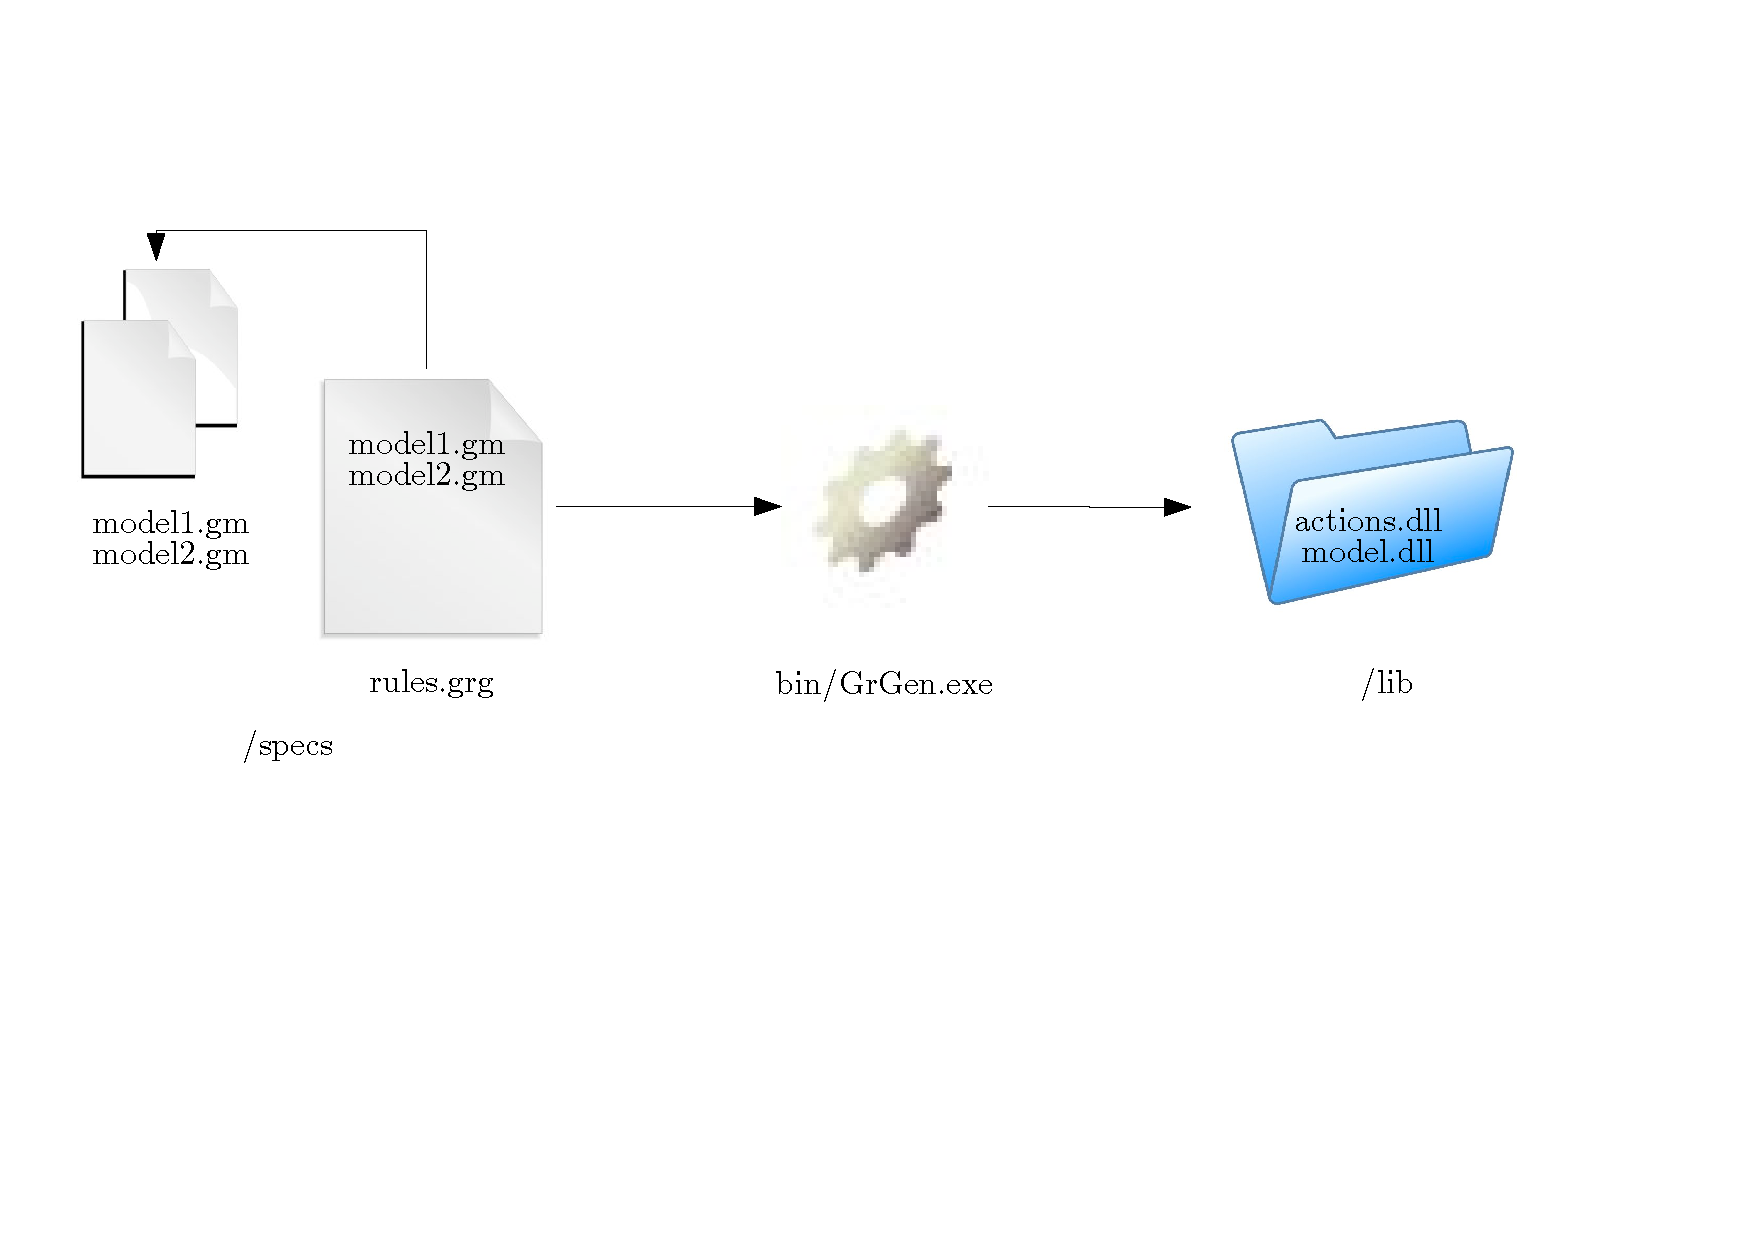
\includegraphics[width=\textwidth]{fig/process}
  \caption{Generating a graph rewriting system}
  \label{process}
\end{figure}

In general you have to distinguish carefully between a graph model (meta level), a host graph, a pattern graph and a rewriting rule. In \GrG\ pattern graphs are implicitly defined by rules, i.e.\ each rule defines its pattern. On the technical side, specification documents for a graph rewriting system can be available as source documents for graph models and rule sets (plain text *.gm and *.grg files) or as their translated .NET modules, either C\# source files or their compiled assemblies (*.dll).


\section{What is Graph Rewriting?}

\begin{figure}[htbp]
	\centering
  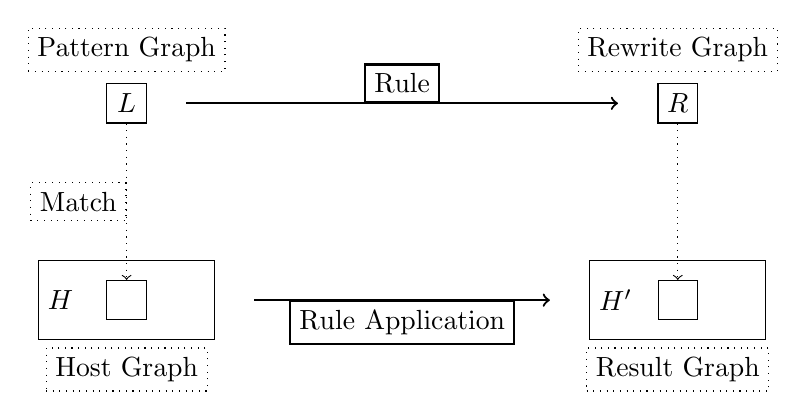
\begin{tikzpicture}
    \begin{scope}[minimum size=0.5cm]
      \tikzstyle{every node}=[draw]
      \node (L)     at (0   ,2.5) {$L$};
      \node (R)     at (7   ,2.5) {$R$};
      \node (mL)    at (0   ,0) {};
      \node (mR)    at (7   ,0) {};
      \node[text width=2cm,text badly ragged,minimum size=1cm] (H)     at (0   ,0) {$H$};
      \node[text width=2cm,text badly ragged,minimum size=1cm] (Hs)    at (7   ,0) {$H'$};
    \end{scope}

    \draw[dotted,->] (L) node[above=0.4cm] {Pattern Graph} -> (mL) node[left,midway]  {Match}   node[below=0.6cm] {Host Graph};
    \draw[dotted,->] (R) node[above=0.4cm] {Rewrite Graph} -> (mR)                              node[below=0.6cm] {Result Graph};

    \pgfsetshortenstart{0.5cm}
    \pgfsetshortenend{0.5cm}
    \draw[thick,->]  (L) -> (R)  node[above,midway] {Rule};
    \draw[thick,->]  (H) -> (Hs) node[below,midway] {Rule Application};
  \end{tikzpicture}
  \caption{Basic Idea of Graph Rewriting}
  \label{figrule}
\end{figure}

How does graph rewriting work? \GrG\ implements an SPO-based approach. Given a host graph $H$, each \emph{rewriting rule} $p: L \longrightarrow R$ consists of a pattern $L$ and a transformation specification $R$ in the form of an adopted pattern graph. The process of rewriting searches a match $H_L \unlhd H$ (i.e.\ a graph homomorphism from $L$ to a subgraph of $H$) and rewrites $H_L$ to $R$. Nodes or edges added to $R$ (in comparison to $L$) will be added $H_L$ and nodes or edges deleted in $R$ will be deleted in $H_L$. The homomorphism may not be unique.


\section{An Example}

We'll have a look at a small example. First we use a special case to construct our host graph: an empty pattern always produces exactly one match (independently of the host graph). So starting with an empty host graph $H$ we construct an apple using
\[ p:  \begin{array}[c]{c} 
\includegraphics[width=3cm]{fig/empty} \end{array} \begin{array}[c]{c} \longrightarrow \end{array} \begin{array}[c]{c} 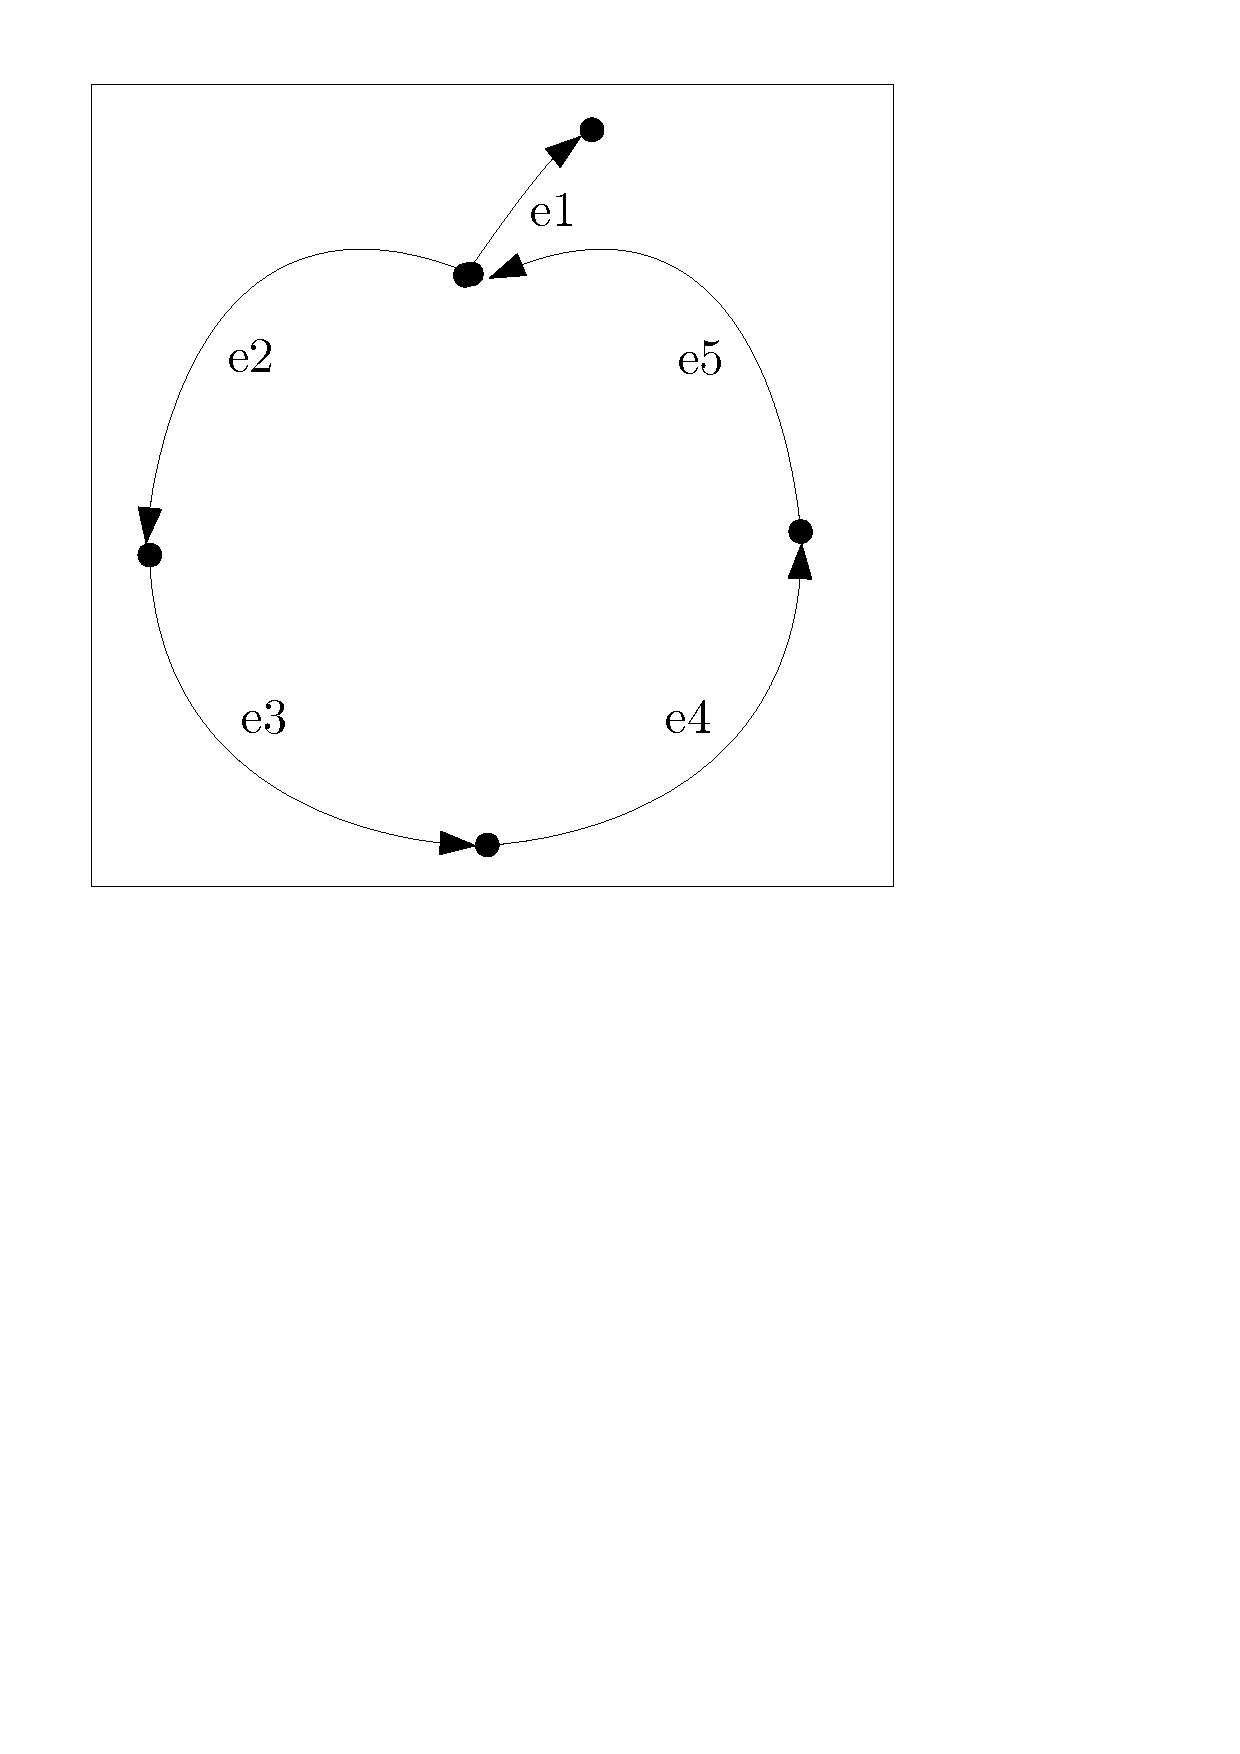
\includegraphics[width=3cm]{fig/apple} \end{array} \]
applied to $H$. We'll get the apple as new host graph $H'$. Now we want to rewrite our apple with stem to an apple with a leaflet. We use
\[ p':  \begin{array}[c]{c} 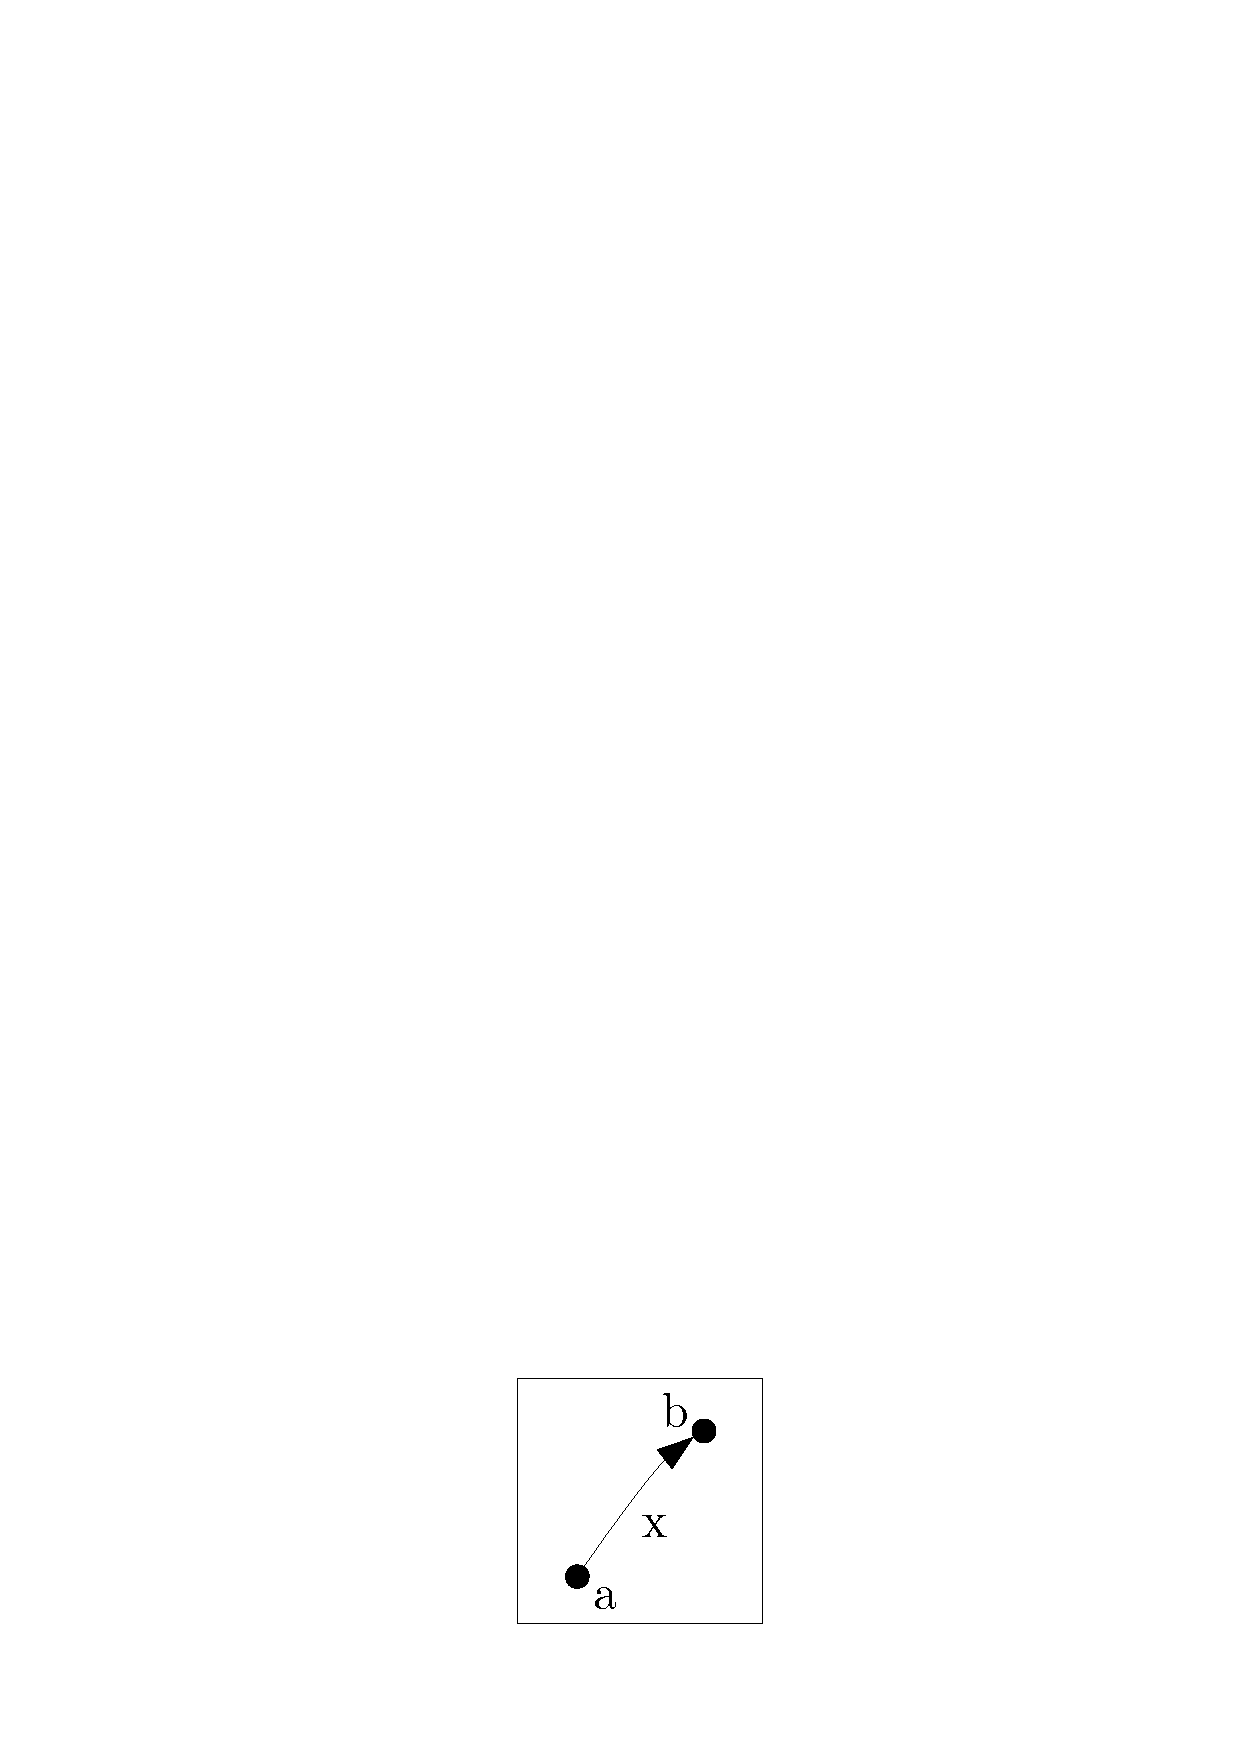
\includegraphics[height=1.25cm]{fig/stiel} \end{array} \begin{array}[c]{c} \longrightarrow \end{array} \begin{array}[c]{c} 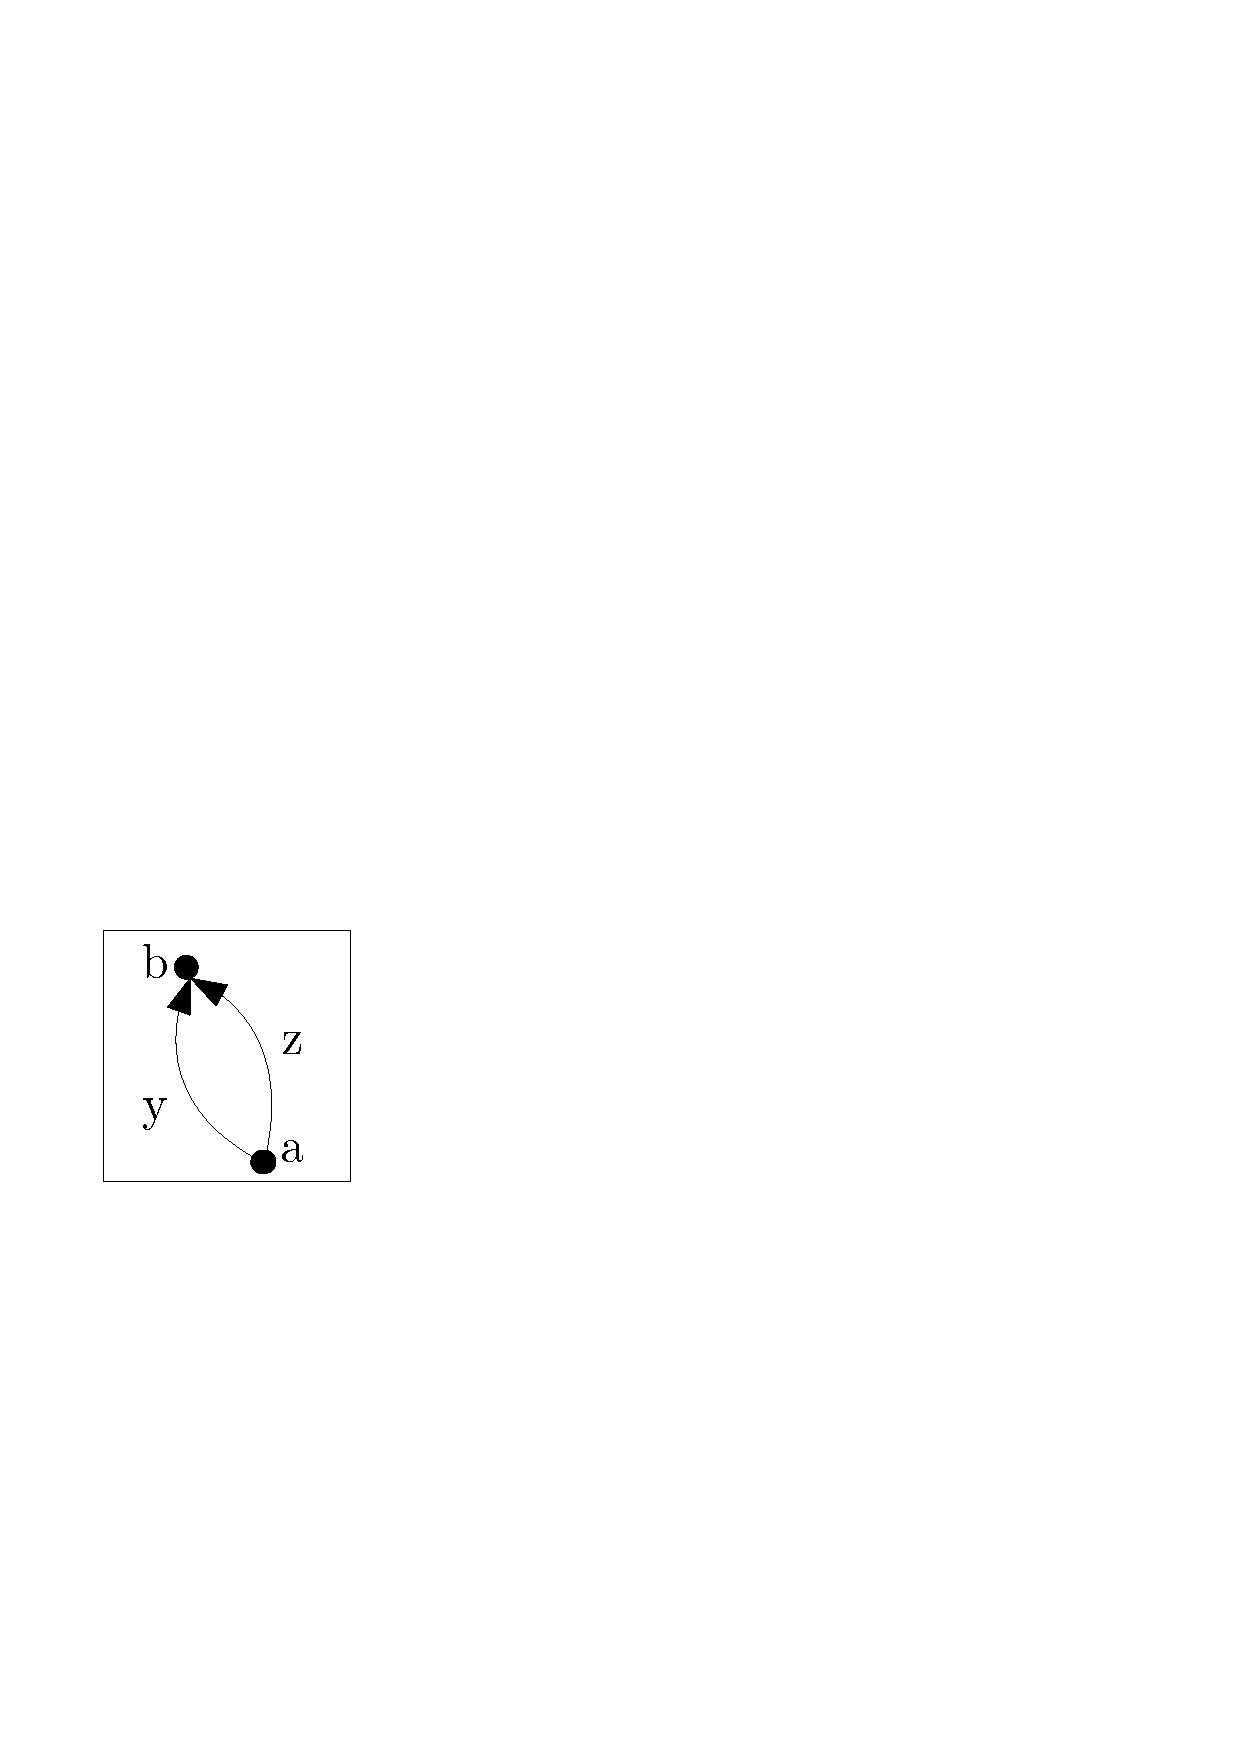
\includegraphics[height=1.25cm]{fig/blatt} \end{array}, \]
apply $p'$ to $H'$ and get the new host graph $H''$, something like this:
\[ 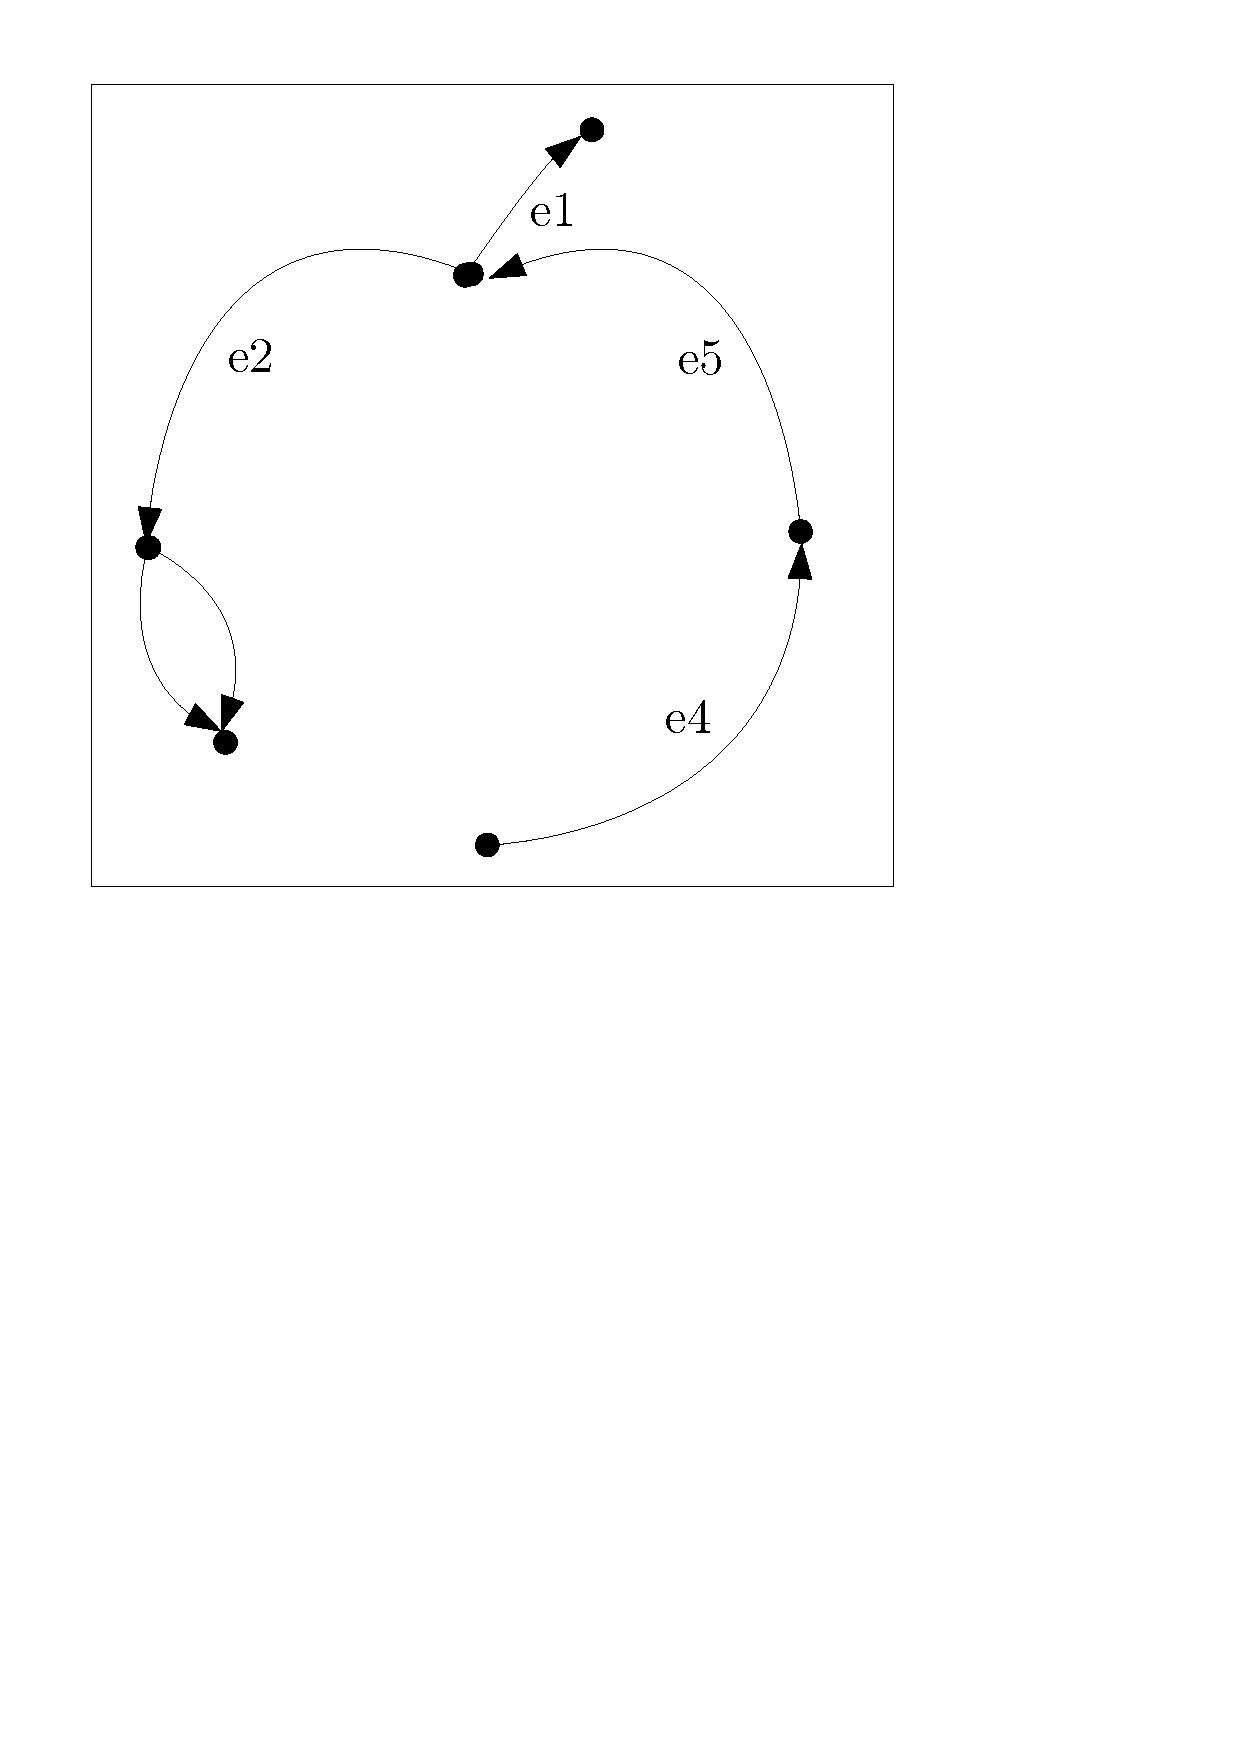
\includegraphics[width=3cm]{fig/wrongapple} \]
What happened? \GrG\ has randomly chosen a match, and $e3$ matches as well as $e1$. A correct solution could make use of edge type information. And this time we'll even keep the stem. So let $H''$ now be
\[ 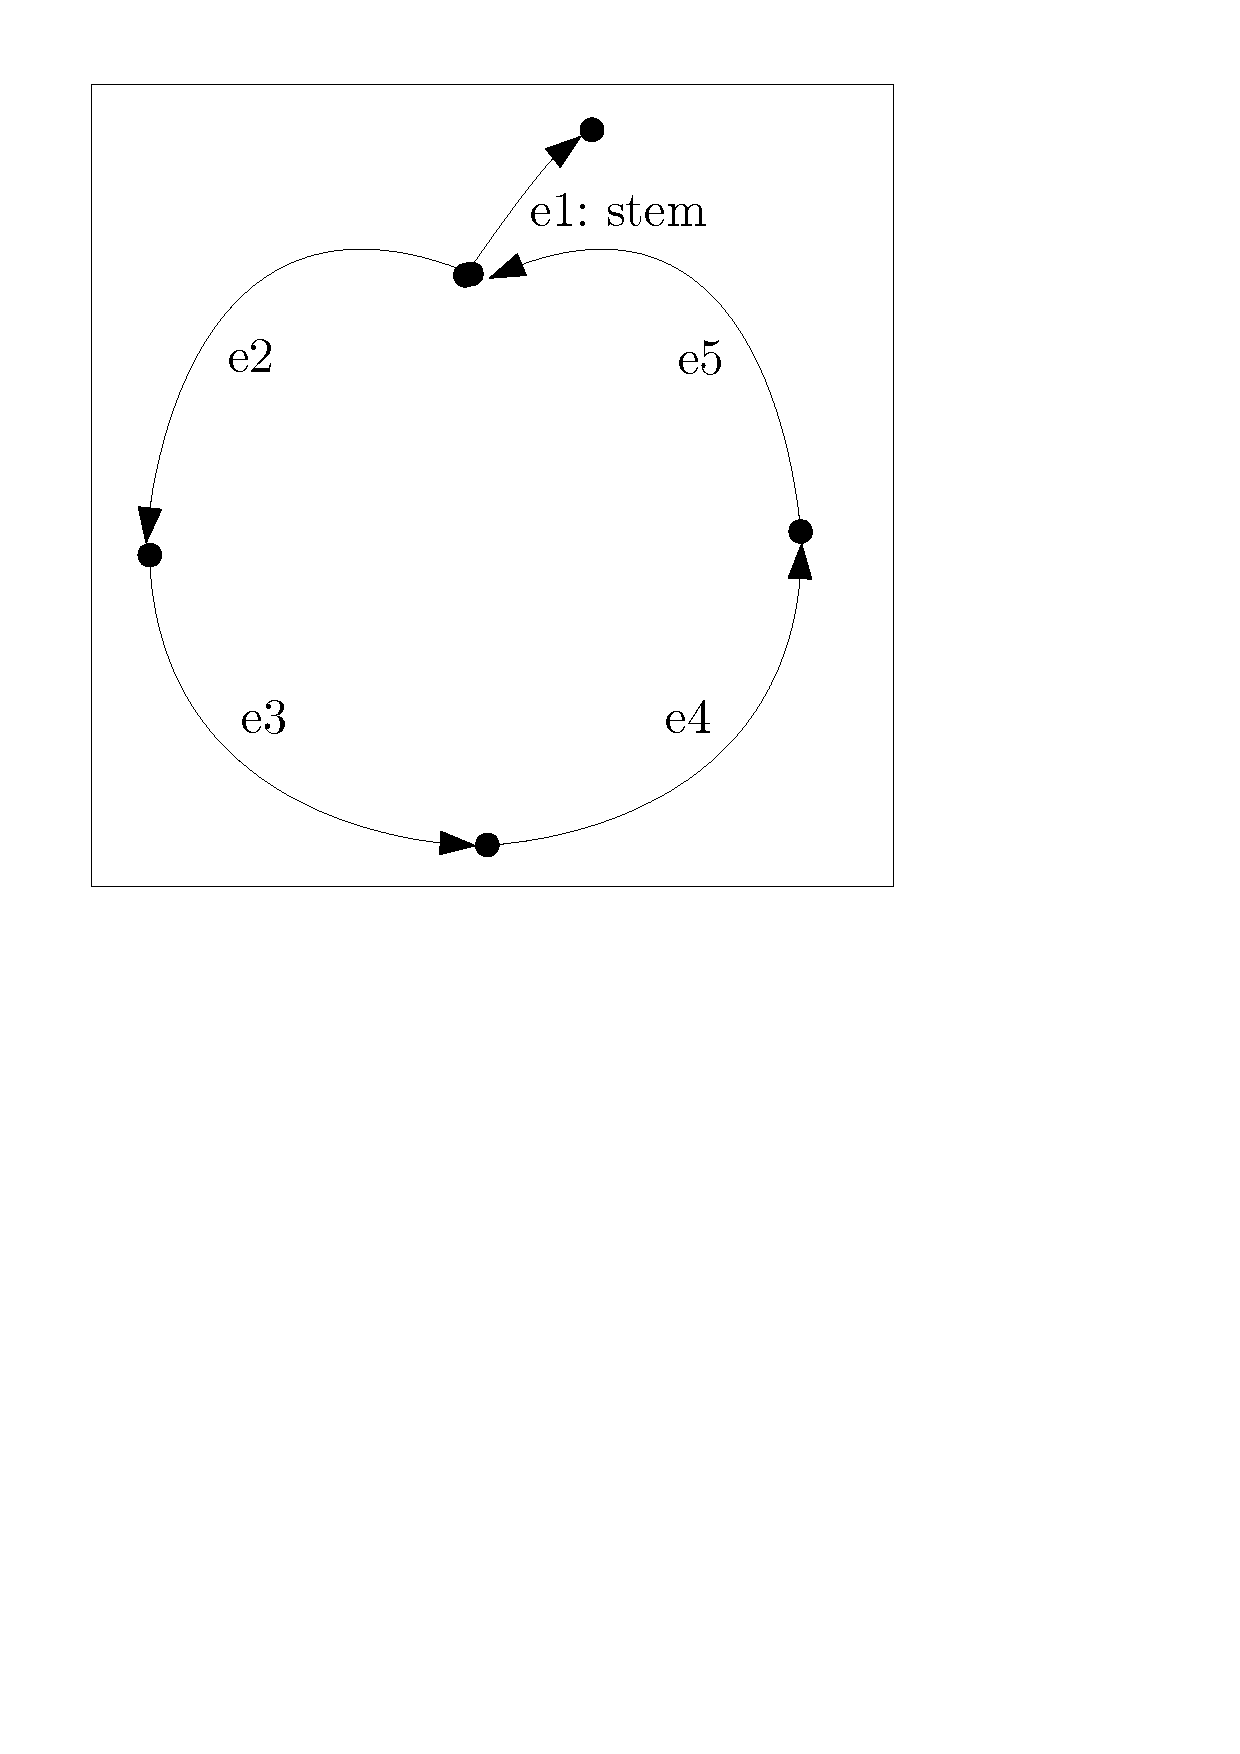
\includegraphics[width=3cm]{fig/typedapple} \]
and
\[ p'':  \begin{array}[c]{c} 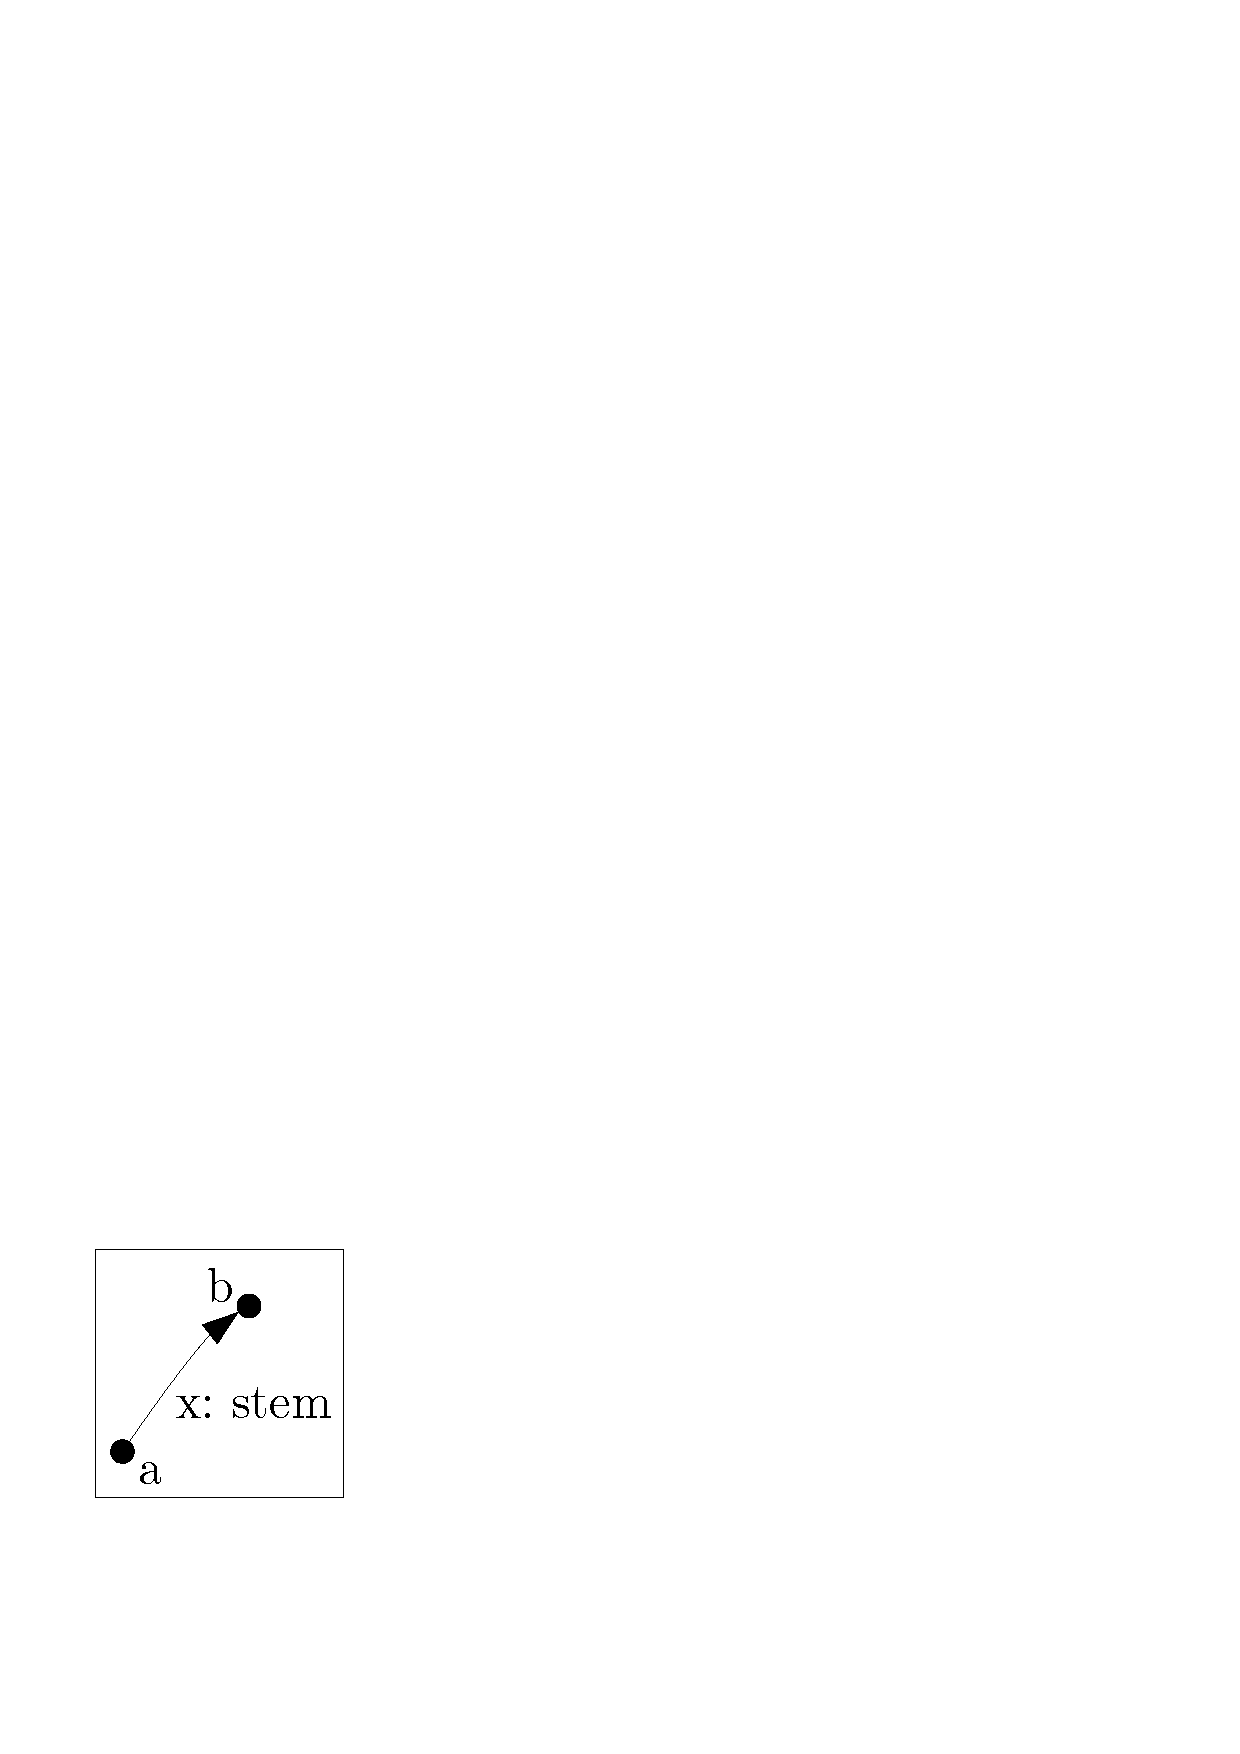
\includegraphics[height=1.25cm]{fig/typedstiel} \end{array} \begin{array}[c]{c} \longrightarrow \end{array} \begin{array}[c]{c} 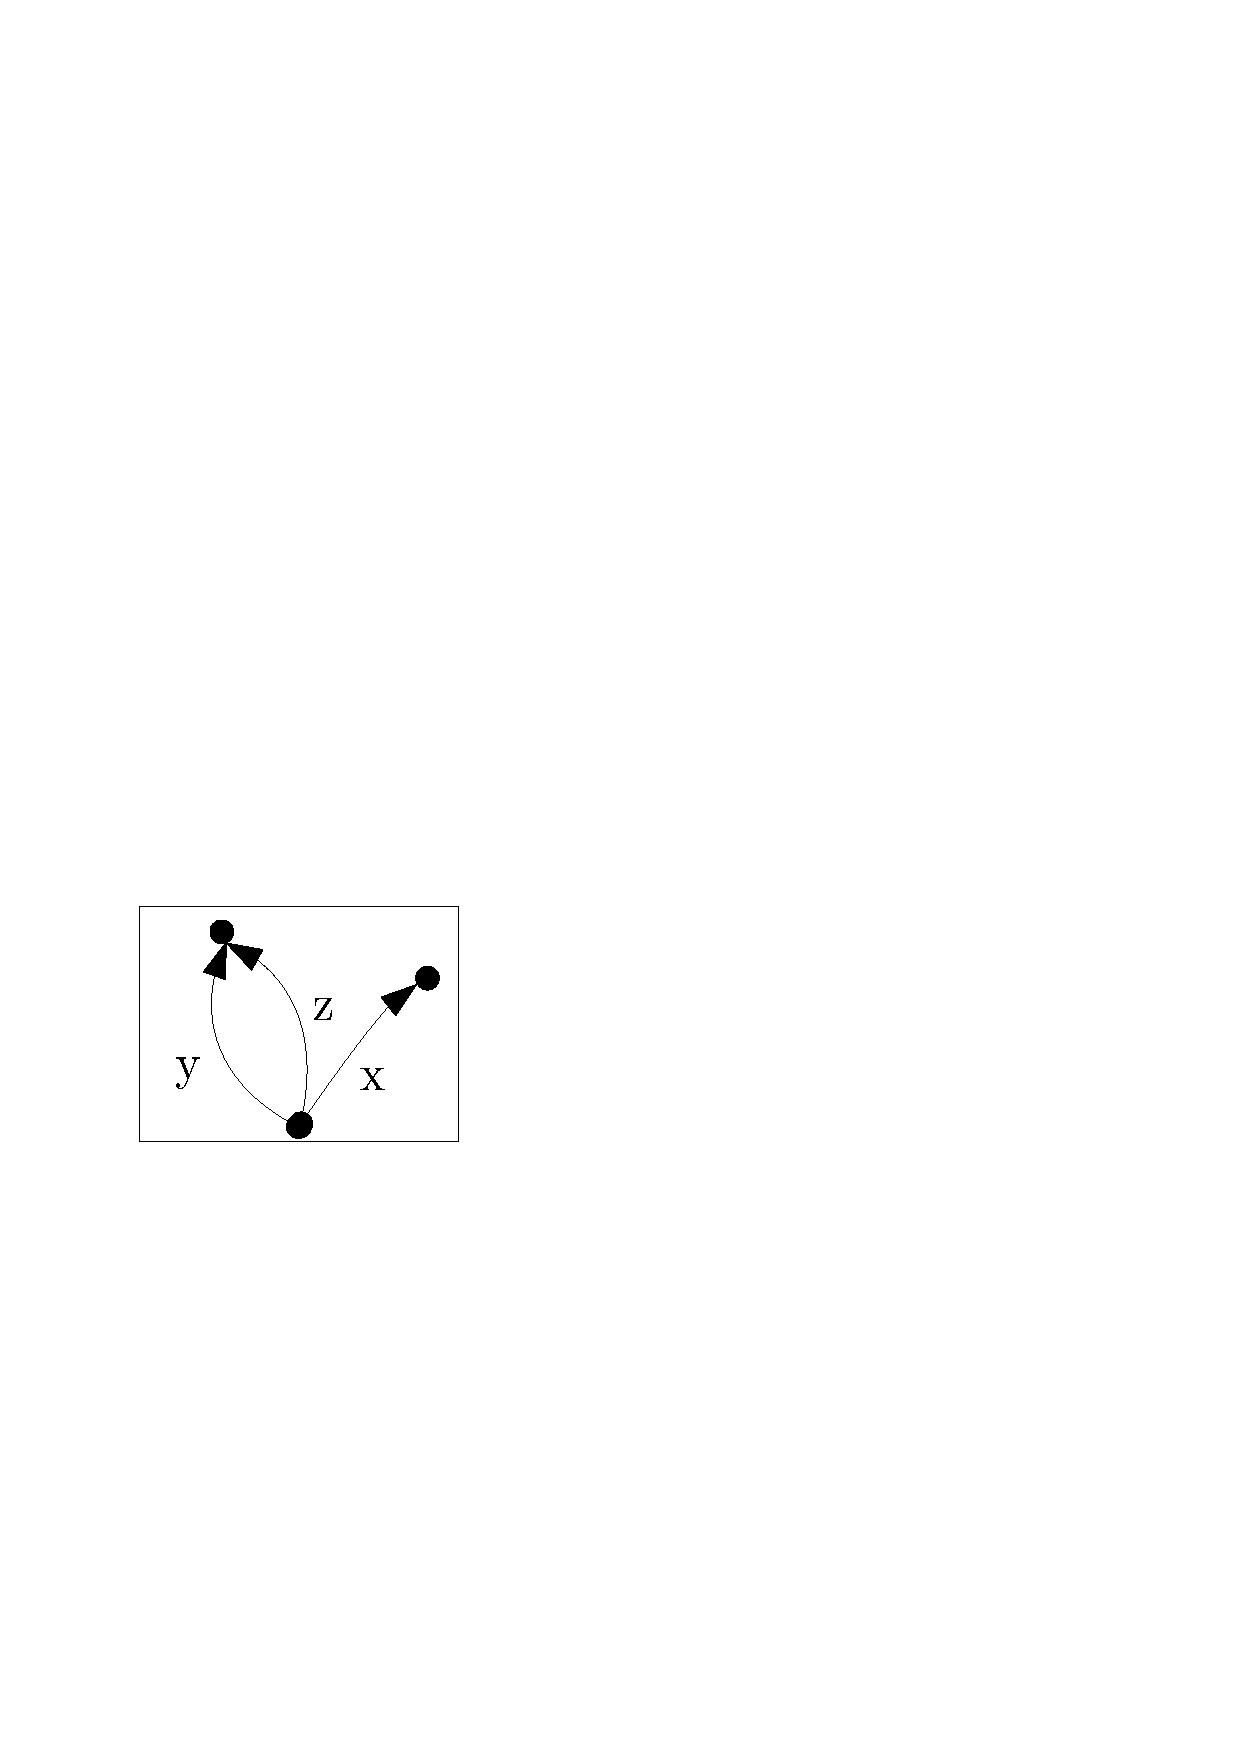
\includegraphics[height=1.25cm]{fig/typedblatt} \end{array}. \]
If we apply $p''$ to $H''$ this leads to
\[ 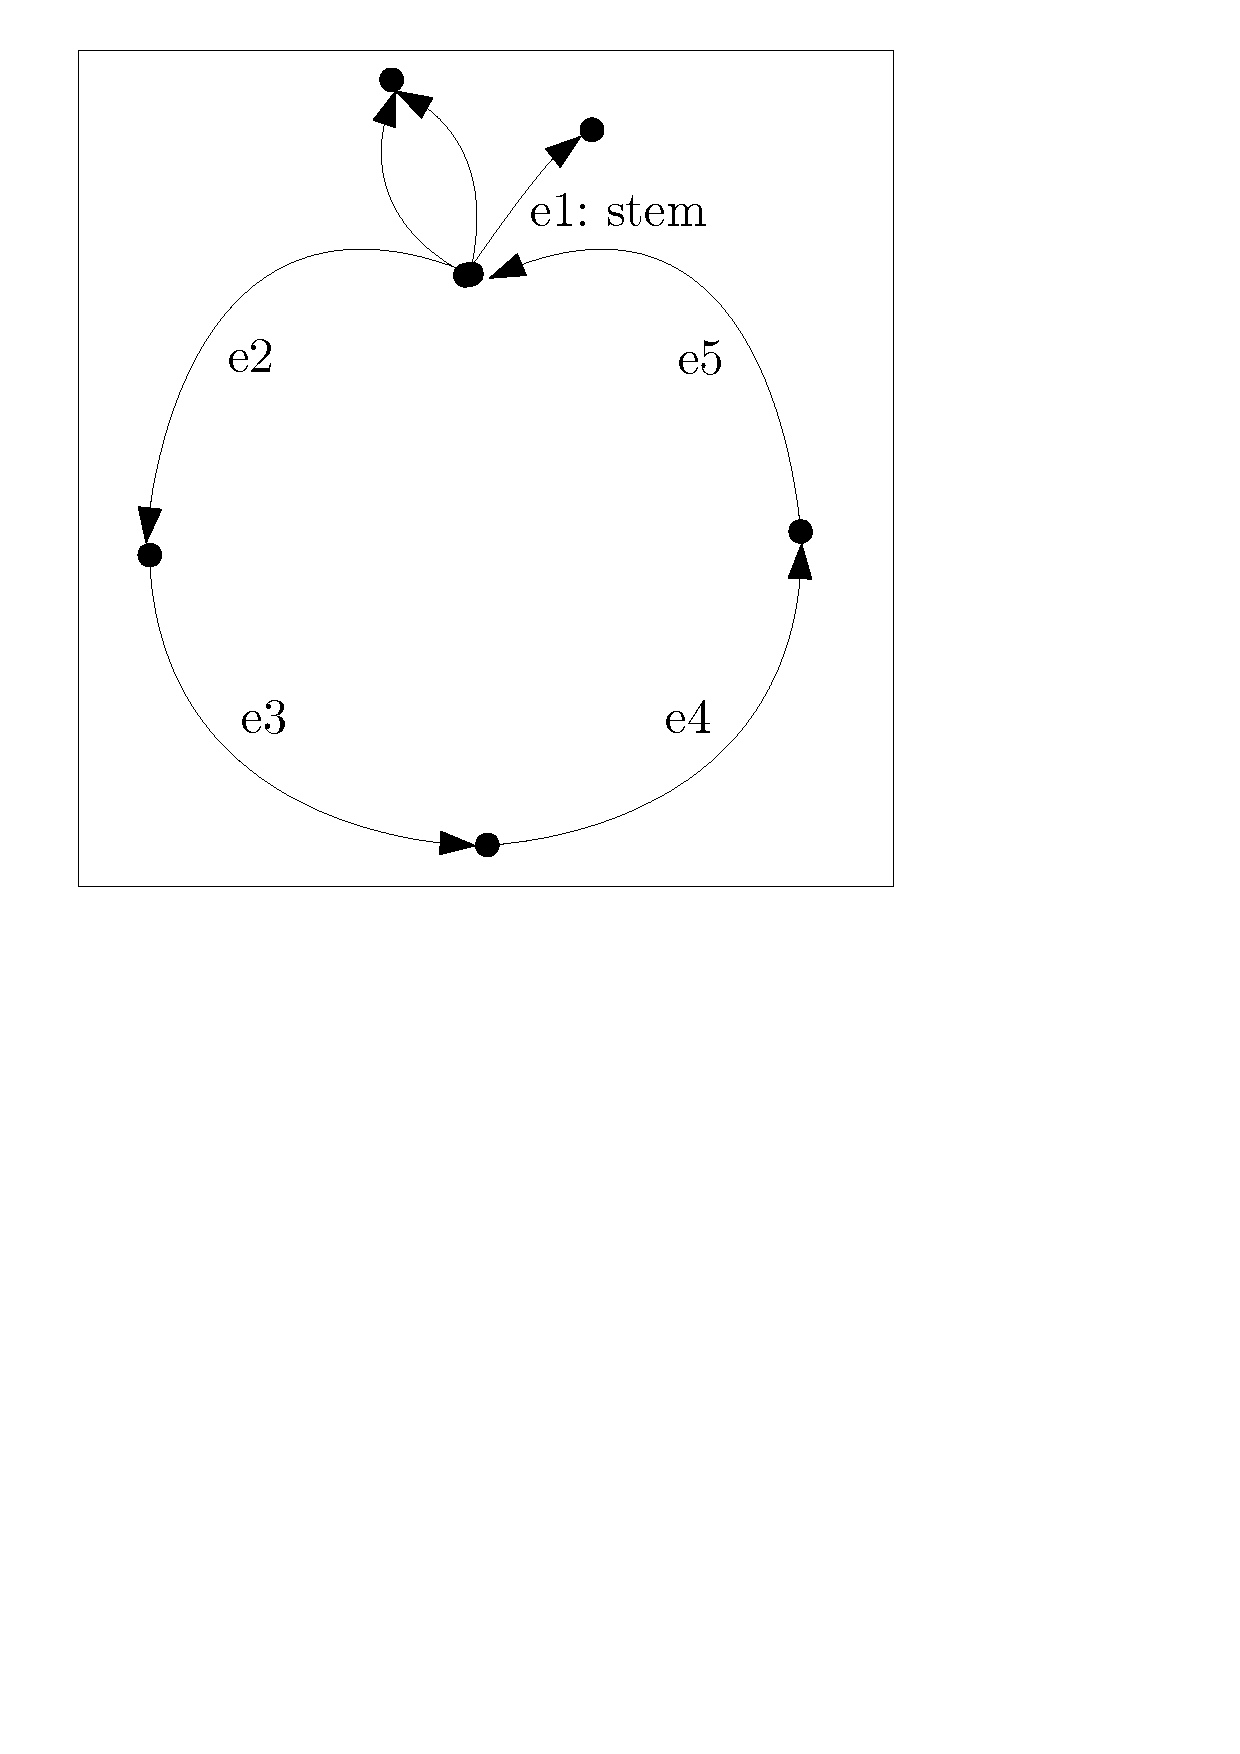
\includegraphics[width=3cm]{fig/rewrittenapple} \]
\emph{Note:} If we had applied $(p')*$ to $H'$ (execute $p'$ consecutively until no match is found) this would not have terminated, because each rewrite had produced one new candidate (one deleted, two added) for matching.    

